\documentclass[11pt]{article}
\usepackage[top=1.5cm,bottom=1.5cm,left=1.5cm,right= 1.5cm]{geometry}
%\geometry{landscape}                % Activate for for rotated page geometry
\usepackage[parfill]{parskip}    % Activate to begin paragraphs with an empty line rather than an indent
\usepackage{graphicx}
\usepackage{amssymb}
\usepackage{epstopdf}
\usepackage{setspace}            
\usepackage{amsmath}            
\usepackage{multirow}    
\usepackage{changepage}
\usepackage{lscape}
\usepackage{ulem}
\usepackage{multicol}
\usepackage{dashrule}
\usepackage[usenames,dvipsnames]{color}       
\usepackage{enumerate}
\newcommand{\urlwofont}[1]{\urlstyle{same}\url{#1}}
\newcommand{\degree}{\ensuremath{^\circ}}

\DeclareGraphicsRule{.tif}{png}{.png}{`convert #1 `dirname #1`/`basename #1 .tif`.png}

\newenvironment{choices}{
\begin{enumerate}[(a)]
}{\end{enumerate}}

\pagestyle{empty}

%\newcommand{\soln}[1]{\textcolor{MidnightBlue}{\textit{#1}}}	% delete #1 to get rid of solutions for handouts
\newcommand{\soln}[1]{ \vspace{2.7cm} }

\newcommand{\solnMult}[1]{\textbf{\textcolor{MidnightBlue}{\textit{#1}}}}	% uncomment for solutions
%\newcommand{\solnMult}[1]{ #1 }	% uncomment for handouts

%\newcommand{\pts}[1]{ \textbf{{\footnotesize \textcolor{black}{(#1)}}} }	% uncomment for handouts
\newcommand{\pts}[1]{ \textbf{{\footnotesize \textcolor{red}{(#1)}}} }	% uncomment for handouts

\newcommand{\note}[1]{ \textbf{\textcolor{red}{[#1]}} }	% uncomment for handouts

\definecolor{oiG}{rgb}{.298,.447,.114}
\definecolor{oiB}{rgb}{.337,.608,.741}

\usepackage[colorlinks=false,pdfborder={0 0 0},urlcolor= oiG,colorlinks=true,linkcolor= oiG, citecolor= oiG,backref=true]{hyperref}

%\usepackage{draftwatermark}
%\SetWatermarkScale{4}

\usepackage{titlesec}
\titleformat{\section}
{\color{oiB}\normalfont\Large\bfseries}
{\color{oiB}\thesection}{1em}{}
\titleformat{\subsection}
{\color{oiB}\normalfont}
{\color{oiB}\thesubsection}{1em}{}

\newcommand{\ttl}[1]{ \textsc{{\LARGE \textbf{{\color{oiB} #1} } }}}

\newcommand{\tl}[1]{ \textsc{{\large \textbf{{\color{oiB} #1} } }}}

\begin{document}

Dr. \c{C}etinkaya-Rundel \hfill Data Analysis and Statistical Inference \\

\ttl{Application exercise: 1.5 Randomization testing} 

\section*{Case study: Student-to-faculty ratio}

Student-to-faculty ratio data collected from random samples of public and private four-year colleges:

\begin{multicols}{2}
\begin{center}
\begin{tabular}{l | c | c}
\hline
		& $public$	& $private$ \\
\hline
$mean$	& 18		& 14 \\
\hline
$sd$		& 4.6		& 7.3 \\
\hline
$n$		& 57		& 85 \\
\end{tabular}
\end{center}

\begin{center}
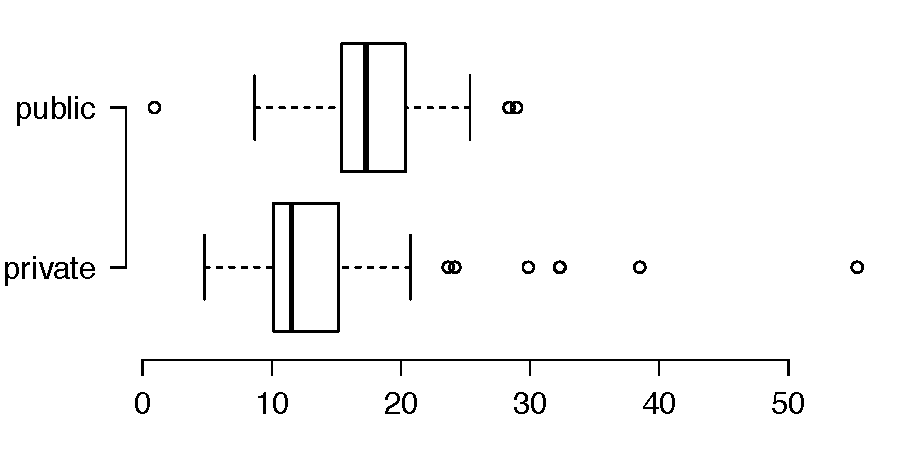
\includegraphics[width=0.4\textwidth]{ratio/ratio_box}
\end{center}
\end{multicols}

\begin{enumerate}

\item We would like to test if there is a \emph{difference} between the average student-to-faculty ratio between public and private four-year colleges using a randomization test. What are the hypotheses?

\item Fill in the blanks below for the appropriate set up for this test:

\begin{doublespace}
We write the student-to-faculty ratio of each public and private college in this sample on a total of \rule{2cm}{0.5pt} index cards. Then, we shuffle these cards and split them into two groups: one group of size \rule{2cm}{0.5pt} representing public colleges, and another group of size \rule{2cm}{0.5pt} representing private colleges. We calculate the difference between the average student-to-faculty ratios in the public and private colleges ($\bar{x}_{public} - \bar{x}_{private}$) and record this value. We repeat this many times to build a randomization distribution, which should be centered at \rule{2cm}{0.5pt} . Lastly, we calculate the p-value as the proportion of simulations where the simulated differences in means are \rule{2cm}{0.5pt}.
\end{doublespace}

\item The dot plot below is created using 100 simulations. What is the p-value?

\begin{center}
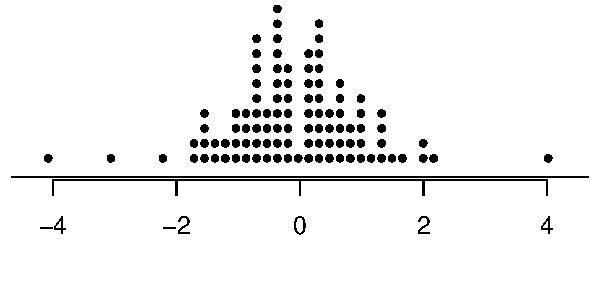
\includegraphics[width=0.6\textwidth]{ratio/rand_dist}
\end{center}

\item Based on the p-value, do these data provide convincing evidence to suggest that the student-to-faculty ratio in public four-year colleges is different than that of private four-year  colleges.

\end{enumerate}

%

\end{document}